\newpage
\setcounter{subsection}{0}
\section{DISEÑO DE LA SOLUCIÓN}

Esta sección presenta la arquitectura del sistema y los artefactos del diseño detallado. La justificación de las tecnologías seleccionadas frente a alternativas se documenta en el anexo de Diseño y Propuesta del Trabajo de Grado.

El diagrama de contexto (Figura~\ref{fig:c4-contexto}) ubica al sistema dentro de su ecosistema: usuarios finales y organizadores interactúan con SecureTicket, que a su vez se comunica con la red Stellar (Soroban RPC y Horizon) y con la billetera Freighter como agente firmante del lado del usuario.

\begin{figure}[H]
\centering
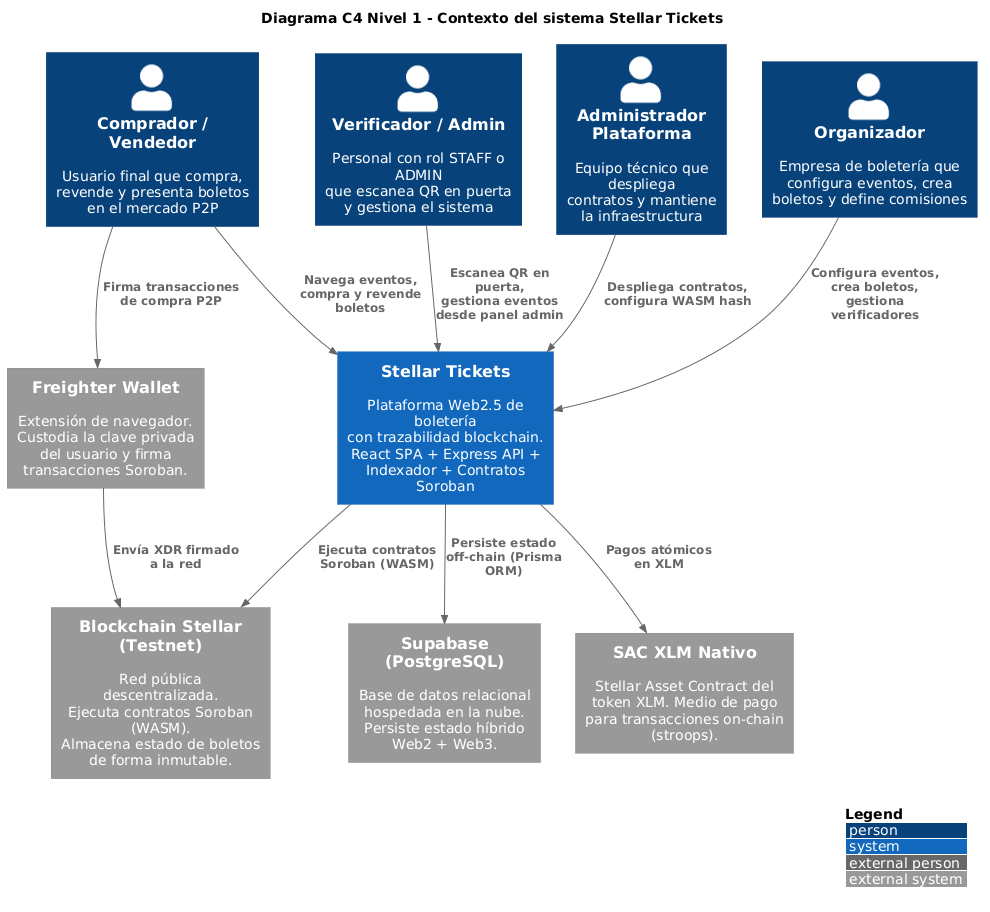
\includegraphics[width=0.95\textwidth]{Imagenes/contextoSecureTicket.png}
\caption{Diagrama de contexto C4 (nivel 1) del sistema SecureTicket.}
\label{fig:c4-contexto}
\end{figure}

\subsection{Actores, roles y límites de confianza}

El sistema separa dos planos de confianza. El plano \textit{on-chain} reúne a los actores que firman operaciones del contrato (organizador, propietario, comprador, verificador, plataforma y administrador del \textit{factory}); todas sus interacciones son validadas por el SCP y registradas en el ledger. El plano \textit{off-chain} reúne al backend, al indexador y a la base de datos relacional. El backend opera bajo un modelo de \textit{proxy XDR stateless}: construye transacciones sin firmar cuando el firmante es el comprador, y firma con la llave del organizador únicamente las operaciones que corresponden a su rol. En ningún momento custodia llaves privadas de usuarios finales.

\subsection{Modelo del ticket NFT}

Cada boleto se modela dentro del contrato de evento mediante la estructura \texttt{Boleto}, cuyos campos se resumen a continuación:

\begin{itemize}\setlength{\itemsep}{2pt}
    \item \texttt{ticket\_root\_id} (tipo \texttt{u32}): identificador estable del boleto a lo largo de todas sus versiones.
    \item \texttt{version} (tipo \texttt{u32}): contador que se incrementa con cada operación de reventa.
    \item \texttt{id\_evento}: identificador del evento al que pertenece el boleto.
    \item \texttt{propietario} (tipo \texttt{Address}): dirección Stellar del dueño actual.
    \item \texttt{precio} (tipo \texttt{i128}): valor en la unidad mínima de XLM para aritmética entera exacta.
    \item Campos de estado booleano: \textit{en\_venta}, \textit{es\_reventa}, \textit{usado} e \textit{invalidado}.
\end{itemize}

La unicidad se garantiza por la clave de almacenamiento compuesta \texttt{Boleto(ticket\_root\_id, version)} y por un contador monotónicamente creciente que asigna los identificadores raíz. La autenticidad se valida mediante la firma del organizador al emitir y por la firma del propietario en cada operación posterior. La trazabilidad se materializa mediante eventos on-chain persistidos por el indexador.

\subsubsection{Identificador y separación de datos sensibles}

El contrato almacena exclusivamente datos operacionales públicos (identificadores, propietario, precio y estados booleanos). Los datos personales del comprador permanecen off-chain en el esquema relacional de PostgreSQL, asociados por el identificador interno del usuario y nunca por la llave privada. La vinculación entre ambas capas se realiza a través de la dirección Stellar que el usuario asocia voluntariamente al conectar la extensión Freighter en su navegador.

\subsubsection{Estados y patrón burn/remint}

El ciclo de vida del boleto se modela mediante tres estados:

\begin{itemize}\setlength{\itemsep}{2pt}
    \item \textbf{ACTIVE}: el boleto ha sido emitido y es válido para el ingreso. Corresponde a la condición en la que ambos indicadores (\textit{usado} e \textit{invalidado}) se encuentran en falso.
    \item \textbf{USED}: un verificador autorizado ha redimido el boleto en puerta mediante la operación correspondiente del contrato.
    \item \textbf{CANCELLED}: el organizador ha invalidado el boleto de forma administrativa por circunstancias excepcionales.
\end{itemize}

En cada operación de reventa se aplica el patrón \textit{burn/remint}: la versión vigente se marca como invalidada y se inserta una nueva entrada con versión incrementada, asignando al comprador como propietario. Un índice de versión actual se actualiza de forma atómica para que las consultas apunten siempre a la versión válida. La Figura~\ref{fig:estados} ilustra las transiciones permitidas entre los tres estados.

\begin{figure}[H]
\centering
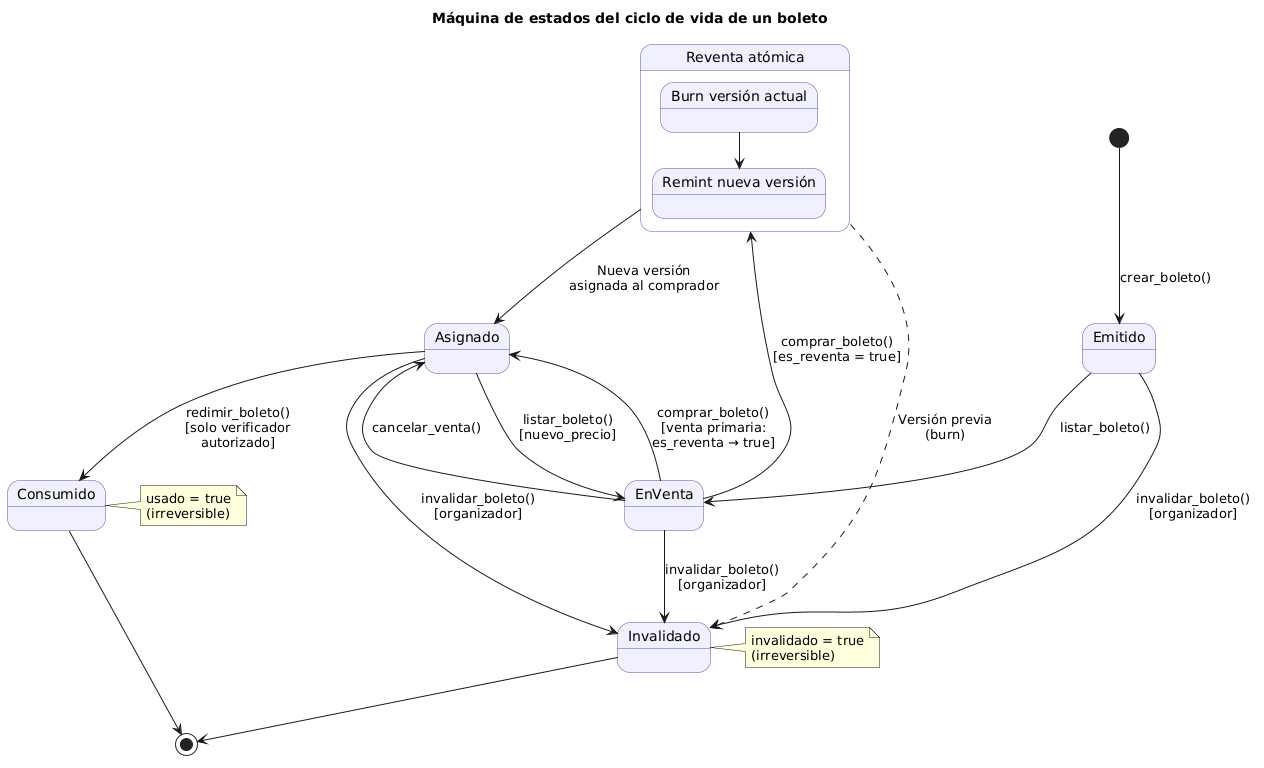
\includegraphics[width=0.95\textwidth]{Imagenes/06_estados_ticket.png}
\caption{Diagrama de estados del boleto: ACTIVE, USED y CANCELLED, con sus transiciones.}
\label{fig:estados}
\end{figure}

\subsection{Diseño de contratos inteligentes}

El sistema utiliza tres contratos Soroban con responsabilidades acotadas: \texttt{factory\_contract}, \texttt{event\_contract} y \texttt{ticket\_nft\_contract}. Esta separación responde al principio de aislamiento de fallos: el estado de cada evento queda confinado a su propio par de contratos y la lógica de emisión NFT se desacopla de las reglas comerciales.

\subsubsection{Contrato Factory}

El contrato \texttt{factory\_contract} implementa el patrón \textit{Factory} para desplegar una instancia independiente del contrato de evento por cada evento creado en la plataforma. Su estructura de configuración agrupa los parámetros necesarios para la inicialización:

\begin{itemize}\setlength{\itemsep}{2pt}
    \item Identificador del evento, dirección del organizador y token de pago.
    \item Porcentajes de comisión (organizador y plataforma) y sus respectivas direcciones de cobro.
    \item Capacidad total del aforo.
\end{itemize}

La función de creación requiere doble autenticación (administrador del \textit{factory} y organizador) y emite el evento \textit{EventoCreado} al completarse. Internamente, el despliegue utiliza la primitiva del entorno Soroban que permite derivar un nuevo contrato a partir del hash WASM registrado, aplicando un \textit{salt} determinístico para garantizar direcciones reproducibles.

\subsubsection{Contrato de Evento}

El contrato \texttt{event\_contract} expone el conjunto funcional principal del sistema. Las funciones utilizan identificadores en español como decisión de trazabilidad académica. La Tabla~\ref{tab:funciones-evento} resume las operaciones disponibles, clasificadas por tipo.

\begin{table}[H]
\centering
\small
\renewcommand{\arraystretch}{1.3}
\definecolor{rowgray}{gray}{0.96}
\caption{Operaciones del contrato de evento.}
\label{tab:funciones-evento}
\begin{tabularx}{\textwidth}{>{\raggedright\arraybackslash}p{2.2cm} >{\raggedright\arraybackslash}p{3.8cm} >{\raggedright\arraybackslash}X}
\toprule
\rowcolor{rowgray}
\textbf{Tipo} & \textbf{Operación} & \textbf{Descripción} \\
\midrule
Inicialización & \texttt{inicializar} & Configura el contrato con los parámetros del evento. \\
\rowcolor{rowgray}
Emisión & \texttt{crear\_boleto} & Acuña un nuevo boleto NFT para un comprador. \\
Reventa & \texttt{listar\_boleto} & Publica un boleto en el mercado secundario. \\
\rowcolor{rowgray}
Reventa & \texttt{cancelar\_venta} & Retira el boleto del mercado secundario. \\
Reventa & \texttt{comprar\_boleto} & Ejecuta la compra atómica (primaria o reventa). \\
\rowcolor{rowgray}
Verificación & \texttt{agregar\_verificador} & Registra un verificador autorizado en puerta. \\
Verificación & \texttt{remover\_verificador} & Revoca la autorización de un verificador. \\
\rowcolor{rowgray}
Redención & \texttt{redimir\_boleto} & Marca el boleto como usado en el ingreso al evento. \\
Administración & \texttt{invalidar\_boleto} & Cancela un boleto por decisión del organizador. \\
\rowcolor{rowgray}
Consultas & \textit{(conjunto de solo lectura)} & Estado, versión, listados y historial del evento. \\
\bottomrule
\end{tabularx}
\end{table}

La operación de compra distingue dos flujos según el estado del boleto:

\begin{itemize}\setlength{\itemsep}{2pt}
    \item \textbf{Venta primaria:} el 100\,\% del precio se transfiere al organizador y el boleto queda habilitado para futuras reventas.
    \item \textbf{Reventa:} el contrato calcula tres montos sobre el precio listado --- comisión del organizador (5\,\%), comisión de plataforma (3\,\%) y monto neto del vendedor (92\,\%) --- y ejecuta las tres transferencias junto con el cambio de propiedad dentro de la misma invocación transaccional.
\end{itemize}

La aritmética de porcentajes utiliza una base entera de 100 (tipo \texttt{i128}) para evitar pérdida de precisión por truncamiento. Las comisiones se validan en la inicialización del contrato para que su suma no supere el 100\,\%.

\subsubsection{Contrato NFT}

El contrato \texttt{ticket\_nft\_contract} proporciona la representación SEP-41-compatible \cite{sep41} del boleto como activo no fungible en un contrato dedicado (aproximadamente 12\,KB de WASM, 10 pruebas unitarias). Expone tres operaciones principales:

\begin{itemize}\setlength{\itemsep}{2pt}
    \item \textit{Mint}: acuña un nuevo NFT vinculado a un propietario, un identificador raíz y una URL de metadatos.
    \item \textit{Transfer}: transfiere la propiedad del NFT entre dos direcciones.
    \item \textit{Burn}: destruye el NFT asociado a un identificador específico.
\end{itemize}

Cada evento despliega su propia instancia de este contrato, en correspondencia uno a uno con su contrato de evento. El identificador del token NFT se renueva en cada reventa para que las referencias almacenadas en la billetera Freighter del propietario anterior no sirvan como prueba válida en puerta.

\subsubsection{Errores tipados y eventos on-chain}

El contrato define dieciséis códigos de error tipados y siete eventos on-chain que el indexador consume para sincronizar la base de datos relacional. Las Tablas~\ref{tab:errores-contrato} y~\ref{tab:eventos-contrato} documentan ambos conjuntos.

\begin{table}[H]
\centering
\small
\renewcommand{\arraystretch}{1.3}
\definecolor{rowgray}{gray}{0.96}
\caption{Códigos de error del contrato de evento.}
\label{tab:errores-contrato}
\begin{tabularx}{\textwidth}{>{\centering\arraybackslash}p{1.0cm} >{\raggedright\arraybackslash}p{4.0cm} >{\raggedright\arraybackslash}X}
\toprule
\rowcolor{rowgray}
\textbf{Cód.} & \textbf{Identificador} & \textbf{Condición de disparo} \\
\midrule
1 & YaInicializado & Intento de reinicializar un contrato activo. \\
\rowcolor{rowgray}
2 & ComisionesMuyAltas & La suma de comisiones supera el 100\,\%. \\
3 & ComisionesNegativas & Algún porcentaje de comisión es negativo. \\
\rowcolor{rowgray}
4 & PrecioInvalido & El precio del boleto es cero o negativo. \\
5 & YaEnVenta & Boleto ya publicado en el mercado secundario. \\
\rowcolor{rowgray}
6 & BoletoUsado & Intento de operar sobre un boleto ya redimido. \\
7 & NoEnVenta & Compra sobre un boleto no listado. \\
\rowcolor{rowgray}
8 & AutoCompra & El propietario intenta comprar su propio boleto. \\
9 & YaUsado & Redención duplicada del mismo boleto. \\
\rowcolor{rowgray}
10 & BoletoNoEncontrado & Identificador o versión inexistente. \\
11 & NoAutorizado & Firma no corresponde al rol requerido. \\
\rowcolor{rowgray}
12 & VersionInvalida & Versión solicitada no coincide con la vigente. \\
13 & BoletoInvalidado & Operación sobre un boleto ya cancelado. \\
\rowcolor{rowgray}
14 & NoInicializado & Contrato invocado antes de su inicialización. \\
15 & VerificadorYaExiste & Registro duplicado de un verificador. \\
\rowcolor{rowgray}
16 & VerificadorNoEncontrado & Revocación de un verificador no registrado. \\
\bottomrule
\end{tabularx}
\end{table}

\begin{table}[H]
\centering
\small
\renewcommand{\arraystretch}{1.3}
\definecolor{rowgray}{gray}{0.96}
\caption{Eventos on-chain emitidos por el contrato de evento.}
\label{tab:eventos-contrato}
\begin{tabularx}{\textwidth}{>{\raggedright\arraybackslash}p{4.5cm} >{\raggedright\arraybackslash}X}
\toprule
\rowcolor{rowgray}
\textbf{Evento} & \textbf{Operación que lo emite} \\
\midrule
\texttt{boleto\_creado} & Acuñación de un nuevo boleto por el organizador. \\
\rowcolor{rowgray}
\texttt{boleto\_listado} & Publicación del boleto en el mercado secundario. \\
\texttt{venta\_cancelada} & Retiro del boleto del mercado secundario. \\
\rowcolor{rowgray}
\texttt{boleto\_comprado\_primario} & Compra en venta primaria completada. \\
\texttt{boleto\_revendido} & Compra en reventa atómica completada. \\
\rowcolor{rowgray}
\texttt{boleto\_redimido} & Redención del boleto en puerta por verificador. \\
\texttt{boleto\_invalidado\_evt} & Cancelación administrativa por el organizador. \\
\bottomrule
\end{tabularx}
\end{table}

\subsection{Arquitectura distribuida (tres nodos)}

El prototipo se despliega en tres nodos lógicos con responsabilidades diferenciadas, lo que permite escalar de forma independiente cada plano y aislar fallos por dominio. La Figura~\ref{fig:c4-contenedores} muestra el diagrama C4 de contenedores con los flujos de datos entre los nodos web, API y datos, y su conexión con la red Stellar.

\begin{figure}[H]
\centering
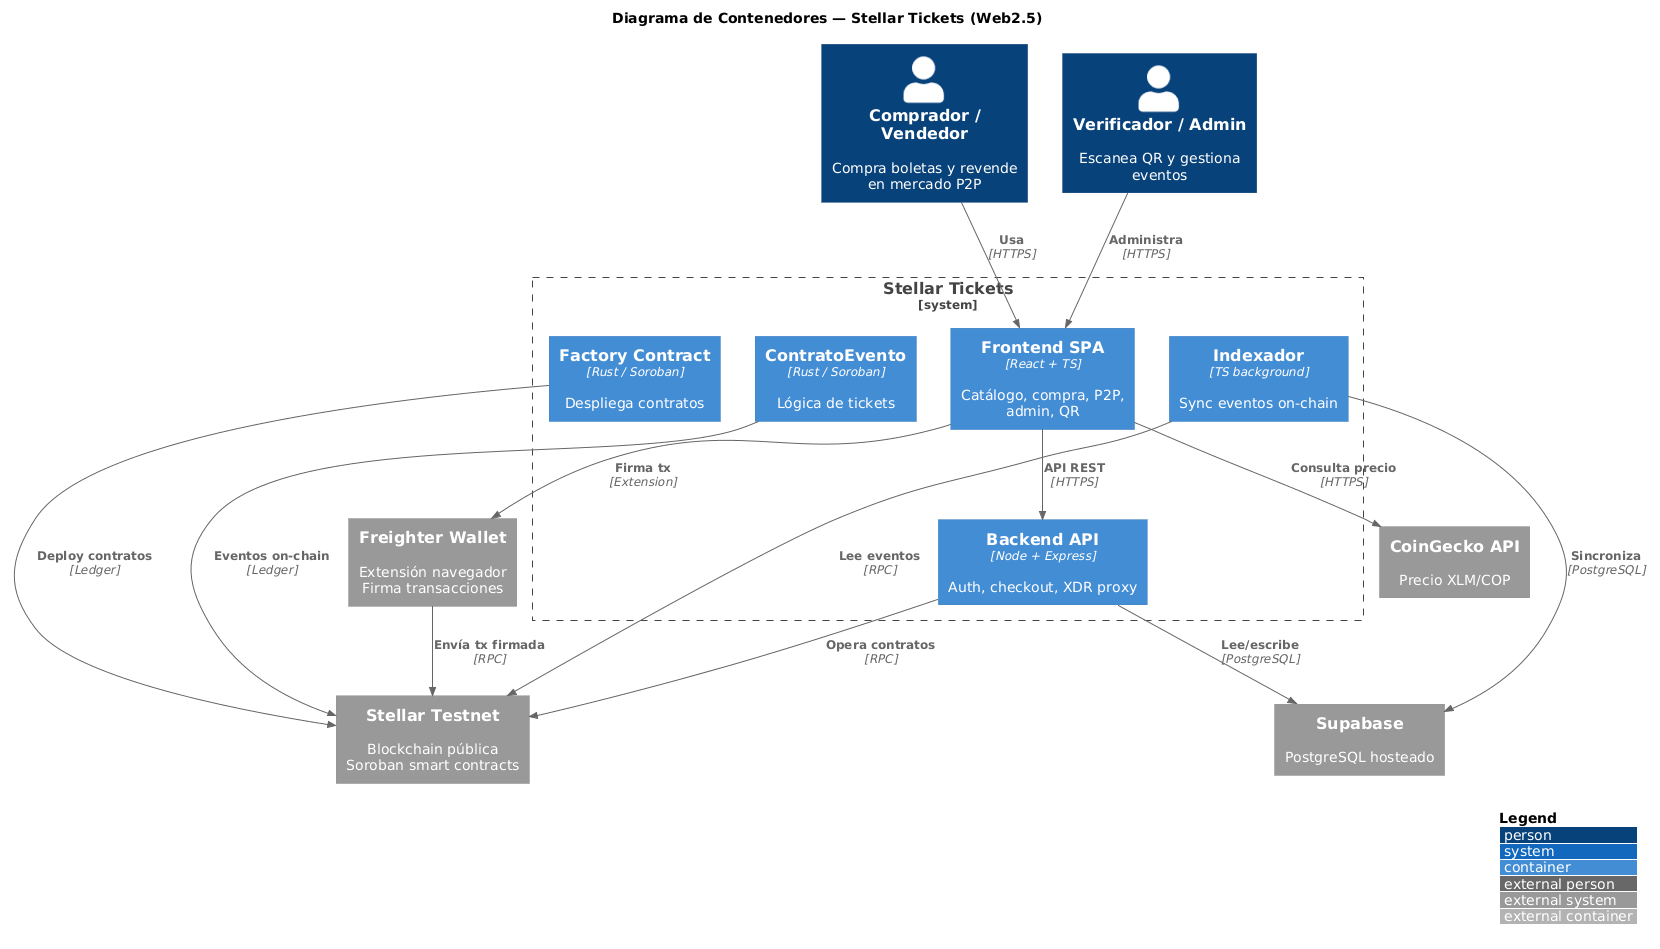
\includegraphics[width=\textwidth]{Imagenes/02_c4_contenedores.png}
\caption{Diagrama C4 de contenedores (nivel 2): nodos web, API y datos, y su acoplamiento con Soroban RPC y Horizon.}
\label{fig:c4-contenedores}
\end{figure}

\subsubsection{Nodo web (frontend)}

Aplicación React~18 con Vite, TypeScript, Tailwind CSS y la familia de componentes shadcn/ui (sobre Radix). La integración Web3 se apoya en dos bibliotecas: \texttt{@stellar/freighter-api} para la firma del comprador y \texttt{@stellar/stellar-sdk} para la construcción local de transacciones de validación. El frontend expone 23 rutas que cubren el flujo de e-commerce (catálogo, carrito, \textit{checkout}, mis entradas y ventas P2P) y los flujos administrativos (panel de gestión y escáner QR).

\subsubsection{Nodo API (backend)}

Backend Node.js con Express y TypeScript, sobre Prisma como ORM contra PostgreSQL. El módulo de autenticación utiliza hashing con factor de costo~10 y tokens JWT con vigencia de 7~días. La integración con Stellar se realiza mediante el SDK oficial en su versión fijada. El backend expone tres familias de endpoints:

\begin{itemize}\setlength{\itemsep}{2pt}
    \item \textbf{Catálogo público:} consultas de eventos y boletos disponibles, con caché en memoria (TTL de 30 a 60 segundos).
    \item \textbf{Autenticación y checkout:} registro, inicio de sesión y flujo de compra primaria con liquidación fiat simulada.
    \item \textbf{Integración Soroban:} construcción de transacciones XDR para asegurar boletos, listar en reventa, cancelar listados, generar la transacción de compra para firma del comprador y enviarla a la red.
\end{itemize}

\subsubsection{Nodo datos (PostgreSQL + indexador)}

La base de datos relacional se hospeda en Supabase bajo el esquema \texttt{ticketing}. El modelo de datos comprende las entidades del dominio Web2 (usuarios, eventos, organizadores, recintos, tipos de boleto, inventario de asientos, carritos, órdenes y pagos) y los campos Web3 añadidos a la tabla de boletos: dirección del contrato, identificador raíz, versión, indicador de venta, precio de reventa (tipo entero largo en la unidad mínima de XLM), dirección del propietario actual y código del activo. La unicidad on-chain se refleja en un índice único compuesto por la dirección del contrato, el identificador raíz y la versión.

El indexador es un proceso de larga duración que consulta el RPC cada 5 segundos. Mantiene un cursor persistente con el último ledger procesado, consume los siete eventos del contrato con semántica idempotente y reposiciona el cursor automáticamente si cae fuera de la ventana de retención del RPC público.

\subsection{Coleccionable Stellar Classic}

Como capa visual adicional, el sistema emite un activo Stellar Classic asociado a cada boleto. El código del activo se compone del prefijo \texttt{T} seguido de 11 caracteres hexadecimales derivados del UUID del boleto. El emisor es la dirección del organizador, configurada con los indicadores de autorización revocable y recuperación habilitada (\textit{clawback}). El flujo opera en cuatro pasos: establecimiento de línea de confianza, envío a la red, emisión idempotente del activo y transferencia mediante recuperación y pago. Esta capa complementa la representación visual del boleto en la billetera del usuario, pero no sustituye al modelo Soroban como fuente de verdad del sistema.
